\section{Description and Methodology}

\subsection{Compiling the Linux kernel}
\begin{figure}[h]
	\centering
	
\includegraphics[width=3cm]{img/uclinux.png}
	\caption{uClinux logo}
	\label{fig:uclinux}
\end{figure}
We were supplied with a variant of Linux called \emph{uClinux}, and it's supplied toolchain. We built the distribution by using a build system named \emph{ptxdist}. We followed \cite[section 5.3]{compendium} step by step, and when done we ended up with a working linux distribuion on the chip, with Tux drawn on the screen. Initially we did not change the kernel config\footnote{We ended up doing so, please see section \ref{subsection:energy-efficiency}.}, nor add any more packages than already supplied and configured.

\subsection{Device driver for the gamepad}
After \emph{uClinux} was installed on the board, the next thing to do was to create a driver for the gamepad. We chose to implement a \emph{platform driver}, which is a more generic way of implementing a driver. It is also the recommended approach.
\subsubsection{Linux kernel module}
\begin{figure}[h]
	\centering
	\lstinputlisting[frame=single, numbers=left]{code/tdt4258_gamepad_driver.c}
	\caption{Driver struct for the \emph{tdt4258\_gamepad\_driver}}
	\label{fig:tdt4258-gamepad-driver}
\end{figure}

A Linux kernel module is a small program that extends the functionality of the kernel. A kernel module runs in kernel space, in contrast to user space, which makes programming the module a little different and more challenging.\\
\\
Since we've chose to implement a \emph{platform driver}, the module init and exit functions does nothing but registering and unregistering the driver with the calls \vn{platform\_driver\_register} and \vn{platform\_driver\_unregister} respectively. The struct used for these calls is shown in figure \ref{fig:tdt4258-gamepad-driver}. The driver initialization is left to the driver probe function, which is described in the following section. 
\subsubsection{Linux character driver}
\paragraph{Innledning om hvordan platform driver fungerer}
Oppsett\\
opprydding
\subsubsection{Character device operations}


\paragraph{Open}
\paragraph{Clone}
\paragraph{Read}
\paragraph{Write}

\subsection{Signals and interrupts}
\label{subsection:signals-and-interrupts}
Based on previous experience regarding energy efficiency, we decided to implement our driver with interrupts and signals right away.
\subsubsection{Enabling and handling interrupts}

Enabling interrupt is done in the \emph{tdt4258\_gamepad\_probe()} method, in the same fashion as the two previous exercises. The only difference is that we write to the specific registers using \emph{iowrite32()} to make the code more portable for virtual memory. For more information about enabling interrupts for the GPIO-controller, see \cite[section 3]{compendium}. We also have to save the IRQ-numbers for the GPIO, for later use. This is done by calling \emph{platform\_get\_irq()} on the platform device that is passed as parameter to the probe function.\\

When a user application calls \emph{open()}, we register the method \emph{gpio\_interrupt\_handler()} as the interrupt handler for the odd and even GPIO PC pins. This is done using the system call \emph{request\_irq()}\footnote{http://www.makelinux.net/books/lkd2/ch06lev1sec3}. The GPIO-handler simply reads and saves the button value and signals the user application that the buttons value has changed. It is also responsible of clearing the interrupt (see \cite[section 3]{compendium} and the code).   

\subsubsection{Generating signals in kernel space}
\begin{figure}[h]
	\centering
	\lstinputlisting[frame=single, numbers=left]{code/signal_user_application.c}
	\caption{Signaling user space from kernel space}
	\label{fig:signal-user-application}
\end{figure}
The \vn{signal\_user\_application()} function in the \mn{driver-gamepad.c} sends a signal to the process who has the driver open. We have used the \textbf{SIGUSR1} signal, because it is documented to be set aside for you to use any way we want and is useful for interprocess communication. In addition to specifying signal type and process to receive the signal, we add the SI\_QUEUE to enable the signal to carry data from kernel to user space. See figure \ref{fig:signal-user-application}.

\subsection{The game application}
Here is a little overview of the files in the game application. There will not be a thorough explanation of the code, as it is well documented.

\begin{itemize}
	\item \mn{game.c} - Main game module. Will initialize signal handlers and external modules, register button and timer handlers and start a \vn{pause()} loop. 
	\item \mn{input.c} - Handles gamepad input. Contains the driver file handle and a list of button handlers. It will determine which button(s) is pressed and/or released, and call the corresponding event handlers.
	\item \mn{pong.c} - This module contains all logic for the Pong game. A more detailed explanation is found in section \ref{subsection:pong}.
	\item \mn{screen.c} - This module handles the screen driver file handle, and takes care of drawing and updating the frame buffer device. A more detailed explanation is found in section \ref{subsection:framebuffer}.
	\item \mn{signal.c} - Module that enables signal handlers for \textbf{SIGALRM} and \textbf{SIGUSR1}. More info about this module is found in section \ref{subsubsection:handling-signals}.
	\item \mn{timer.c} - This module will set up the timer with a given interval, and keep track of which function that should be called on each timer tick. This is needed to animate the game. A more detailed description is found in section \ref{subsubsection:timer}.
\end{itemize}

Most of the C source files have a corresponding header to define their external interfaces.

\subsubsection{The pause() loop}
\begin{figure}[h]
	\centering
	\lstinputlisting[frame=single, numbers=left]{code/pause_loop.c}
	\caption{The pause loop}
	\label{fig:pause-loop}
\end{figure}
The main program will live in a \vn{pause()}\footnote{http://linux.die.net/man/2/pause} loop during execution. This function sleeps until a signal is delivered.

\subsubsection{Timer}
\label{subsubsection:timer}
\begin{figure}[h]
	\centering
	\lstinputlisting[frame=single, numbers=left]{code/setitimer.c}
	\caption{Starting the system timer}
	\label{fig:setitimer}
\end{figure}
The \mn{timer.c} module will start a system timer, using the \vn{setitimer()}\footnote{http://linux.die.net/man/2/setitimer} procedure defined in the C standard library (se figure \ref{fig:setitimer}). On each timer tick, the \textbf{SIGALRM} signal will be sent to the process, which is handeled in \mn{signal.c} and delegated back to \mn{timer.c}.

\subsubsection{Handling signals in user space}
\label{subsubsection:handling-signals}
\begin{figure}[h]
	\centering
	\lstinputlisting[frame=single, numbers=left]{code/sighandler.c}
	\caption{Adding signals handlers with signal mask to the user space}
	\label{fig:sighandler}
\end{figure}
We needed to configure our application \textbf{SIGUSR1} and \textbf{SIGALRM} signals. See figure \ref{fig:sighandler}. The handlers called respective methods in \mn{timer.c} and \mn{input.c}.\\
\\
In other words, with the main program spinning in the \vn{pause()} loop, all of the program work is done entirely by the signal handlers.


\subsection{Controlling the framebuffer device}
\label{subsection:framebuffer}
The EFM32GG has it's own framebuffer device that manages the display. This device is accessed by opening the driver \emph{/dev/fb0} as a file. When the file is opened, we have access to the drivers methods. As described in \cite[section 5.4.2]{compendium}, this means that we can use \emph{read()}, \emph{write()} and \emph{lseek()} wich can be used to handle the frambuffer byte by byte as a usual file. But, as \cite[section 5.4.2]{compendium} describes, there is a way controlling the frambuffer that is easier and faster then using the mentioned method. \\

The framebuffer device can be memory mapped. This means that we can map the driver to an array in memory, which in C means that we are able to write pixels directly with an usual C array. This done by calling the function \emph{mmap()}, wich is a Unix system call declared in the header \emph{sys/mmap.h}. 
Writing to the array will update a buffer holding the pixel values. To write the changes in the framebuffer to the display we use the system call \emph{ioctl()}. \\

\emph{ioctl()} is driver specific system call, and can be used to a various of tasks. In our case, it is to update the changes in the framebuffer. The number of parameters to this function varies depending on the driver, but it needs two parameters to work properly. The first is an file descriptor for an open file. The second, a device dependent request code wich specifies if it is an \emph{in} or \emph{out} parameter, and the size of the list of driver specific parameters in bytes. See the mmap-documentation\footnote{http://man7.org/linux/man-pages/man2/ioctl.2.html} for more information.   
\\

After we are done using the display, it is important to clean up. First we have to undo the memory mapping, wich is done by calling the system call \emph{munmap()} (defined in \emph{sys/mmap}). Second we have to close our connection to the device, wich is done by calling \emph{close()} to the framebuffer driver. \\

Our module \emph{screen.c} is responsible of handling the framebuffer device. We memory map the frambuffer in the module. The module contains methods to initialize the display and close the connection to the device, by calling the functions described in this section. It also contains methods to draw simple elements to the screen, in various ways. See the code for more information. 

\subsubsection{Framebuffer update modes}
\label{subsubsection:framebuffer-update-modes}
Other modules can use \mn{screen.c} to draw rectangular elements on the screen. Each of these method calls require the current and next position of the element. The current position is needed so the sceen can fill it in with the background color (black) before the new position of the element is drawn. The module is constructed to handle this behaviour in different ways, so we could test the performance and energy efficiency of each method.

\paragraph{Full screen update}
This mode will draw both elements, and signal the driver to update the entire screen. This is the most straight-forward way of doing it.

\paragraph{Double screen update}
This mode will draw the first element, then signal the driver to update exactly that area, then draw the second and signal the driver to update this location as well. This mode will update as little of the screen as possible, but might introduce overhead due to the invocation of \vn{ioctl()} twice.

\paragraph{Single screen update}
This mode will draw both elements, then do a calculation of the minimum bounding box of the two elements. This will, depending on distance between the current and next position, update more of the screen that is necessairly, but we are left of with one \vn{ioctl()} call.\\
\\
All of the framebuffer update modes are illustrated in figure \ref{fig:framebuffer-update-modes}.
\\
\begin{figure}
	\label{fig:framebuffer-update-modes}
	\centering
	\textbf{Full screen update} \\
	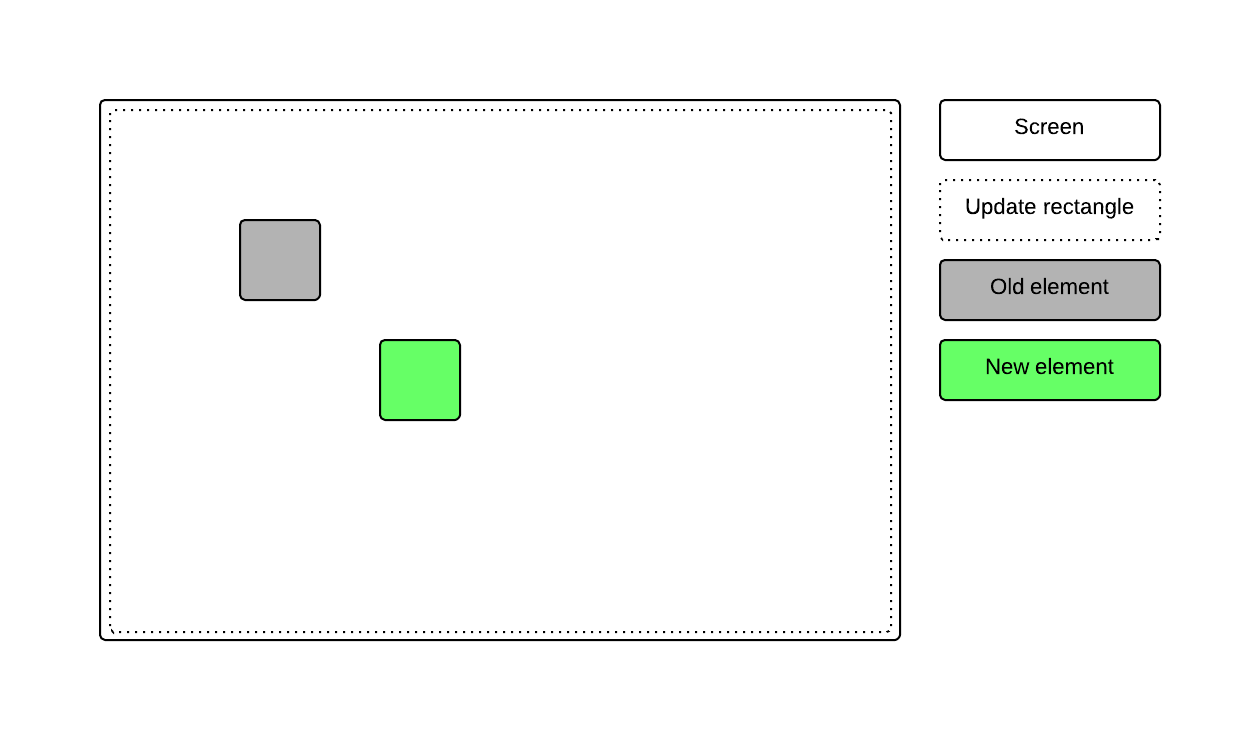
\includegraphics[width=11cm]{img/update_entire_screen.png}\\
	\textbf{Double screen update} \\
	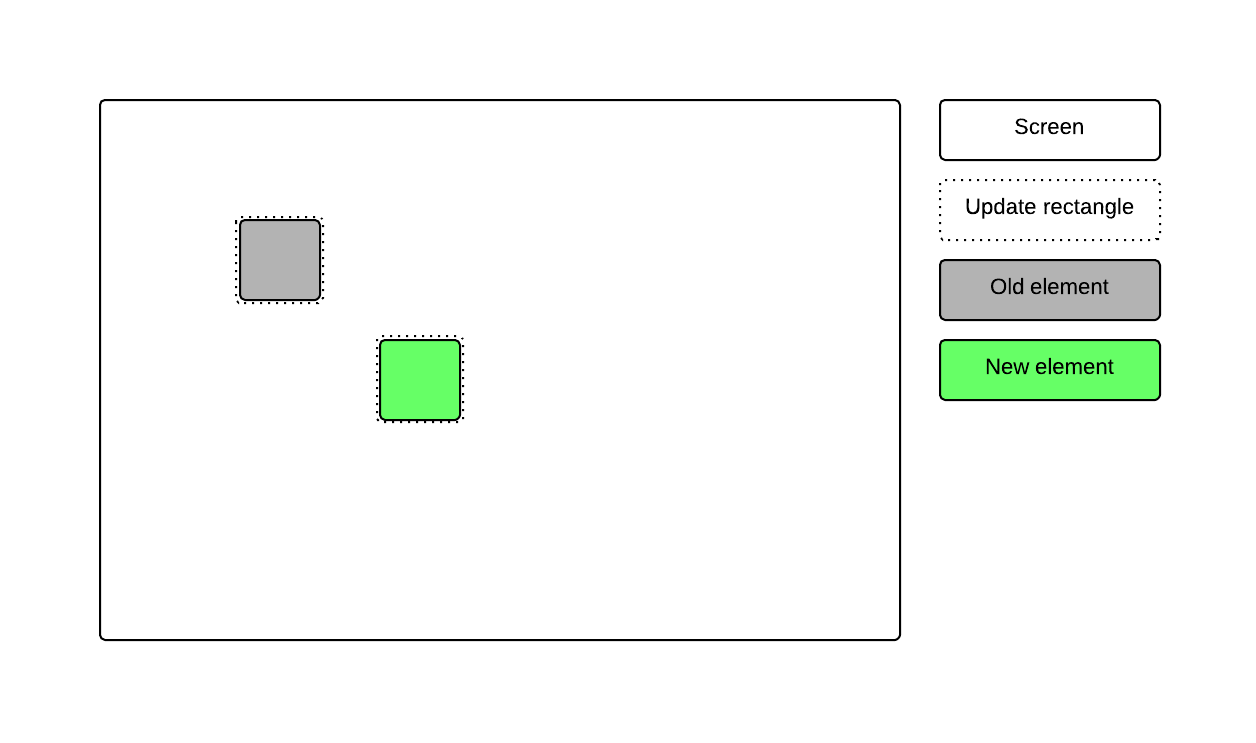
\includegraphics[width=11cm]{img/update_twice.png}\\
	\textbf{Single screen update} \\
	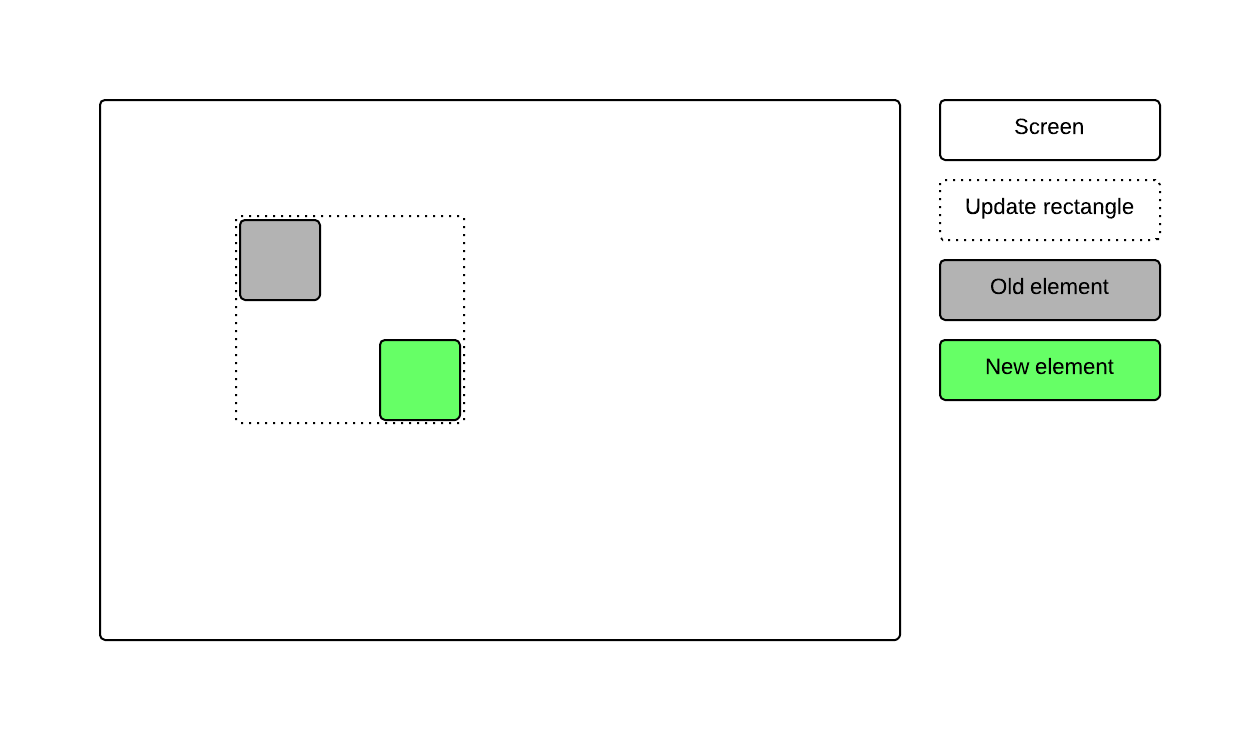
\includegraphics[width=11cm]{img/update_once.png}\\
	\caption{Framebuffer update modes}
\end{figure}
\subsection{Pong}
\label{subsection:pong}
Primarly focusing on the driver, we decided to implement one of the simplest games we know, Pong. Pong is a game simulating table tennis. The players control a virtual paddle each. A ball moves between the paddles until one of the players misses it. The goal is to keep the ball moving until the other player misses the ball.
\begin{figure}[h]
	\label{fig:pong_screenshot}
	\centering
	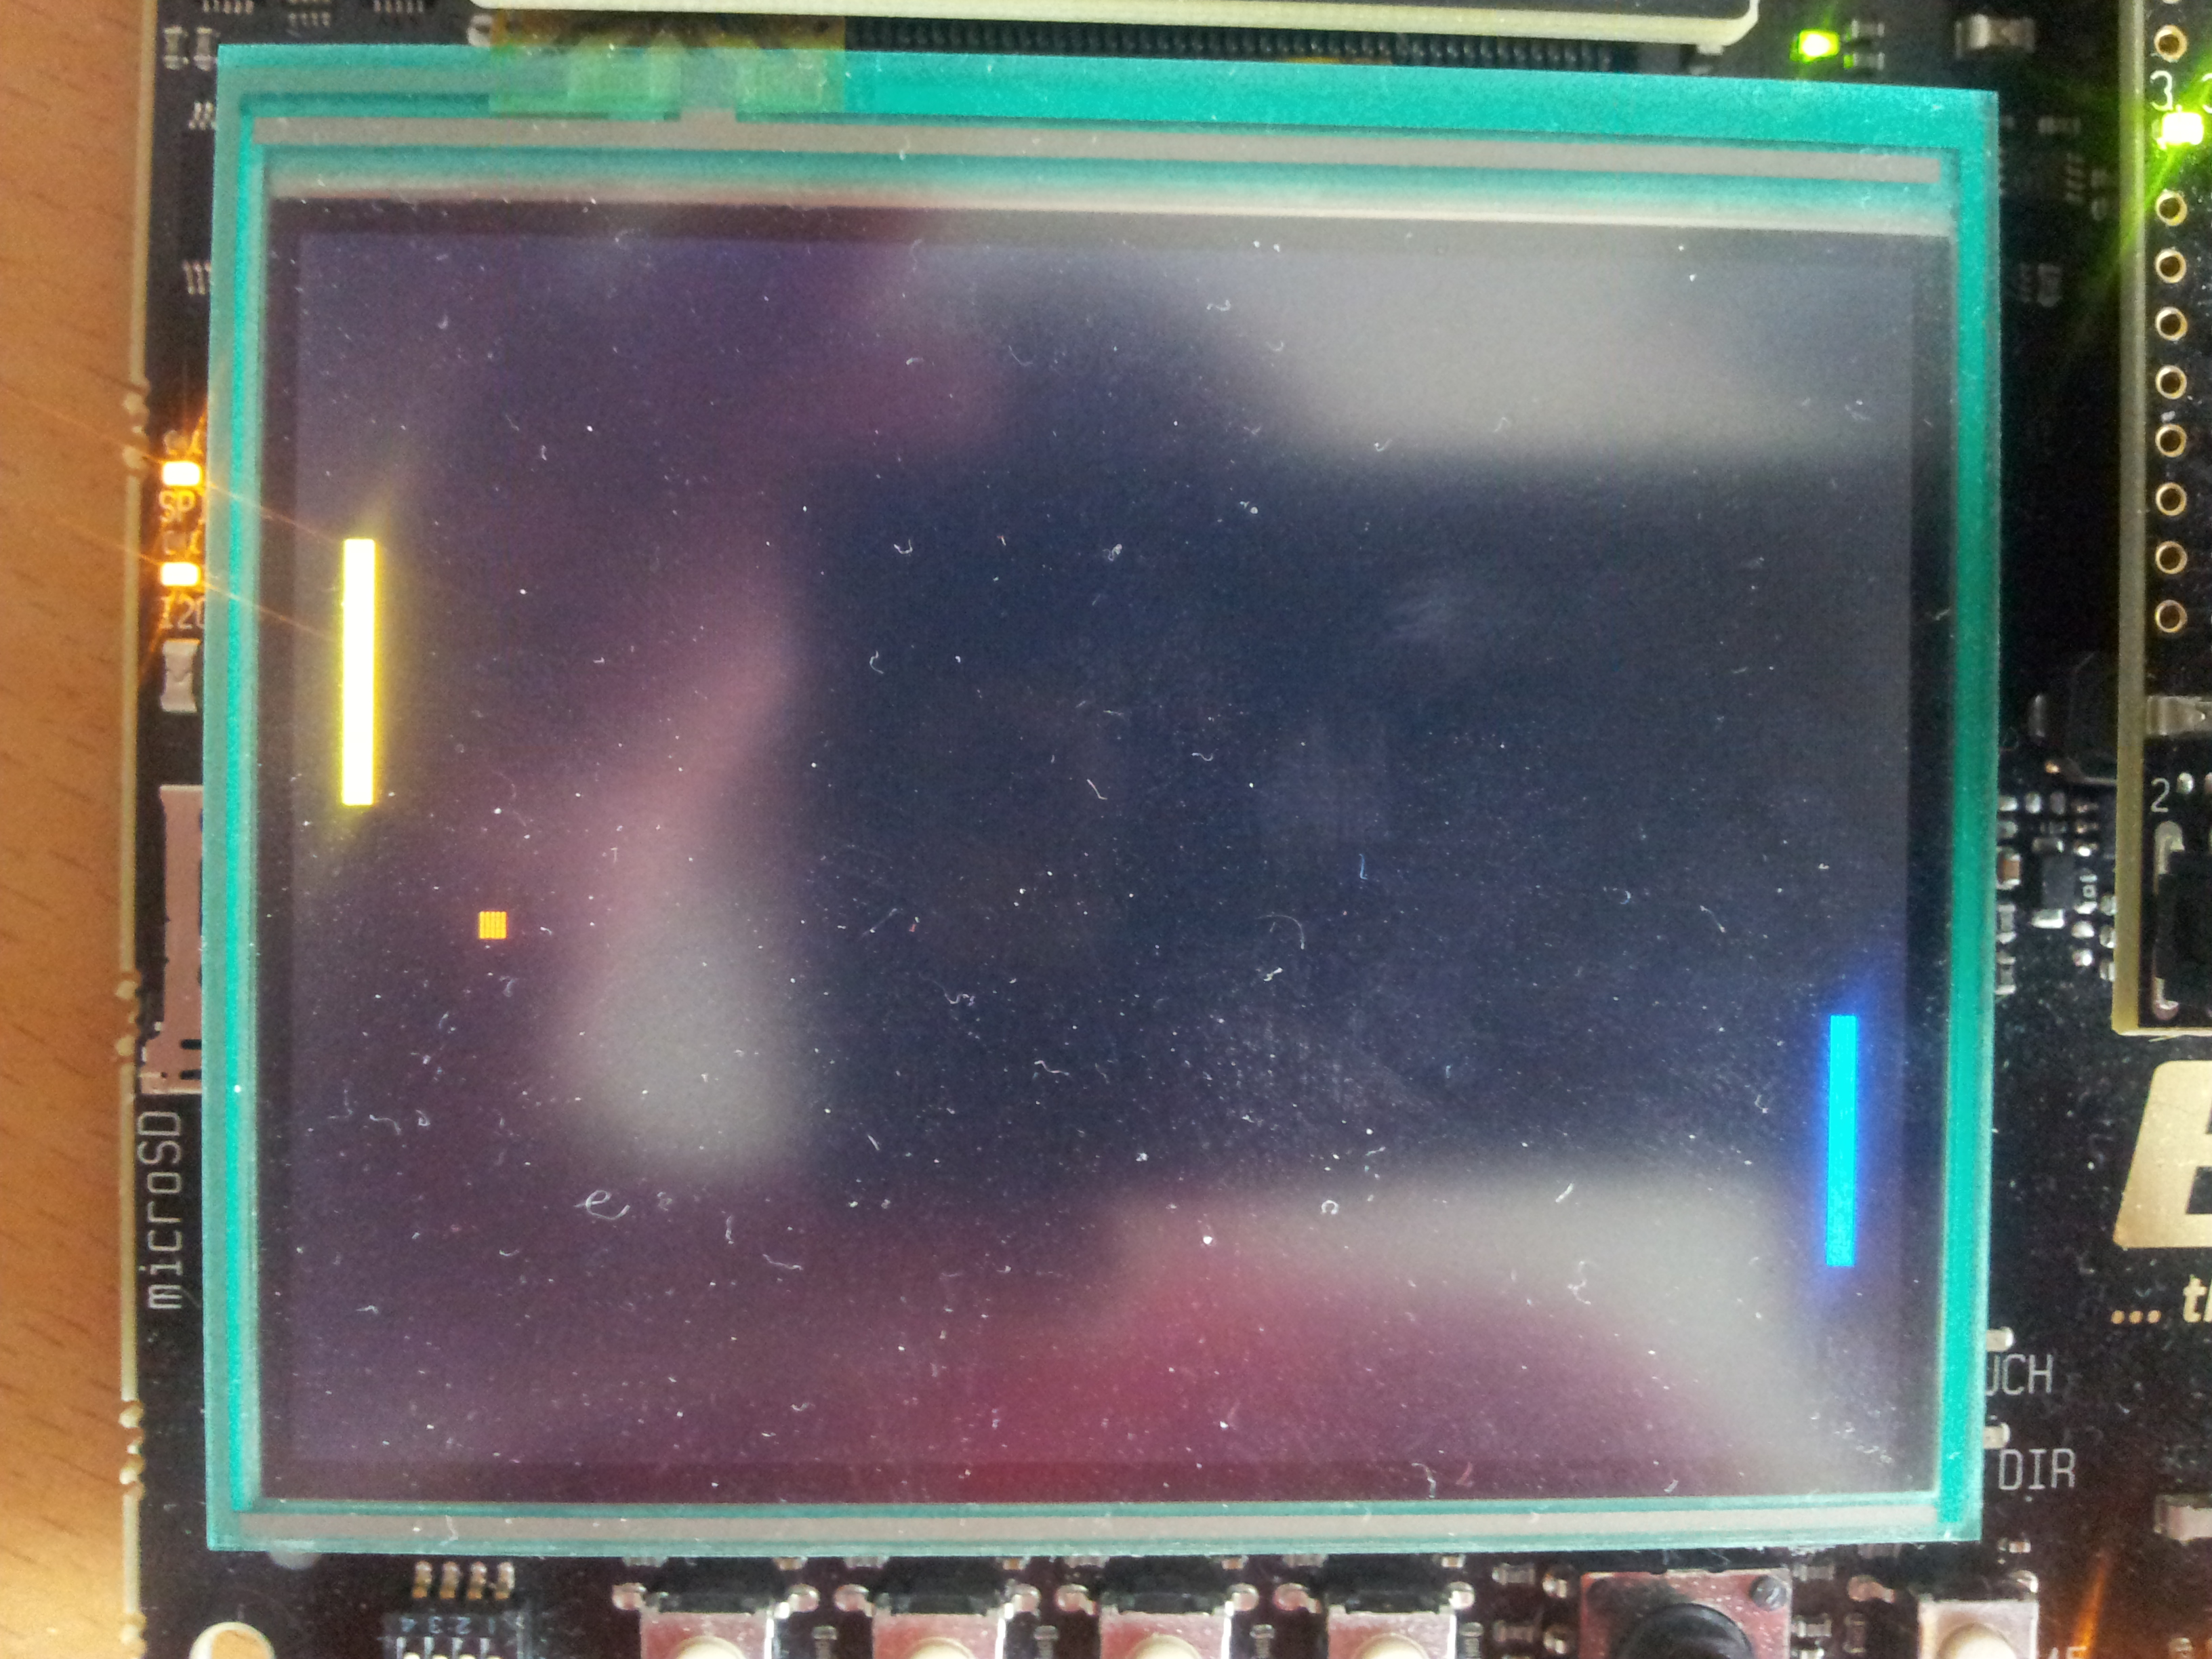
\includegraphics[width=10cm]{img/pong_screen.jpg}
	\caption{Screenshot of the game}
\end{figure}
\paragraph{Implementation} The functions that got called on button press and release adjusted the movement speed of the paddle. When a button got pressed, the speed of the represented player would be set. On release the speed would be set to zero. This way, two calls where needed each time the players moved a paddle. To draw the objects, the game made use of the screen module. A function specified for drawing vertically moving objects where used to draw the player representation. By doing that, the overlapping part would not have to be re-drawn. For simplicitys sake, the screen gets updated at the same time as the positions. This means that an increase in screen update frequency, will also increase the speed of the game. 
\paragraph{Overlapping objects} 
Avoiding overlapping objects became a minor challenge. When the ball overlapped one of the paddles, the overlapping part would go blank when the ball moved away.
\begin{figure}[h]
	\label{fig:pong_overlapping}
	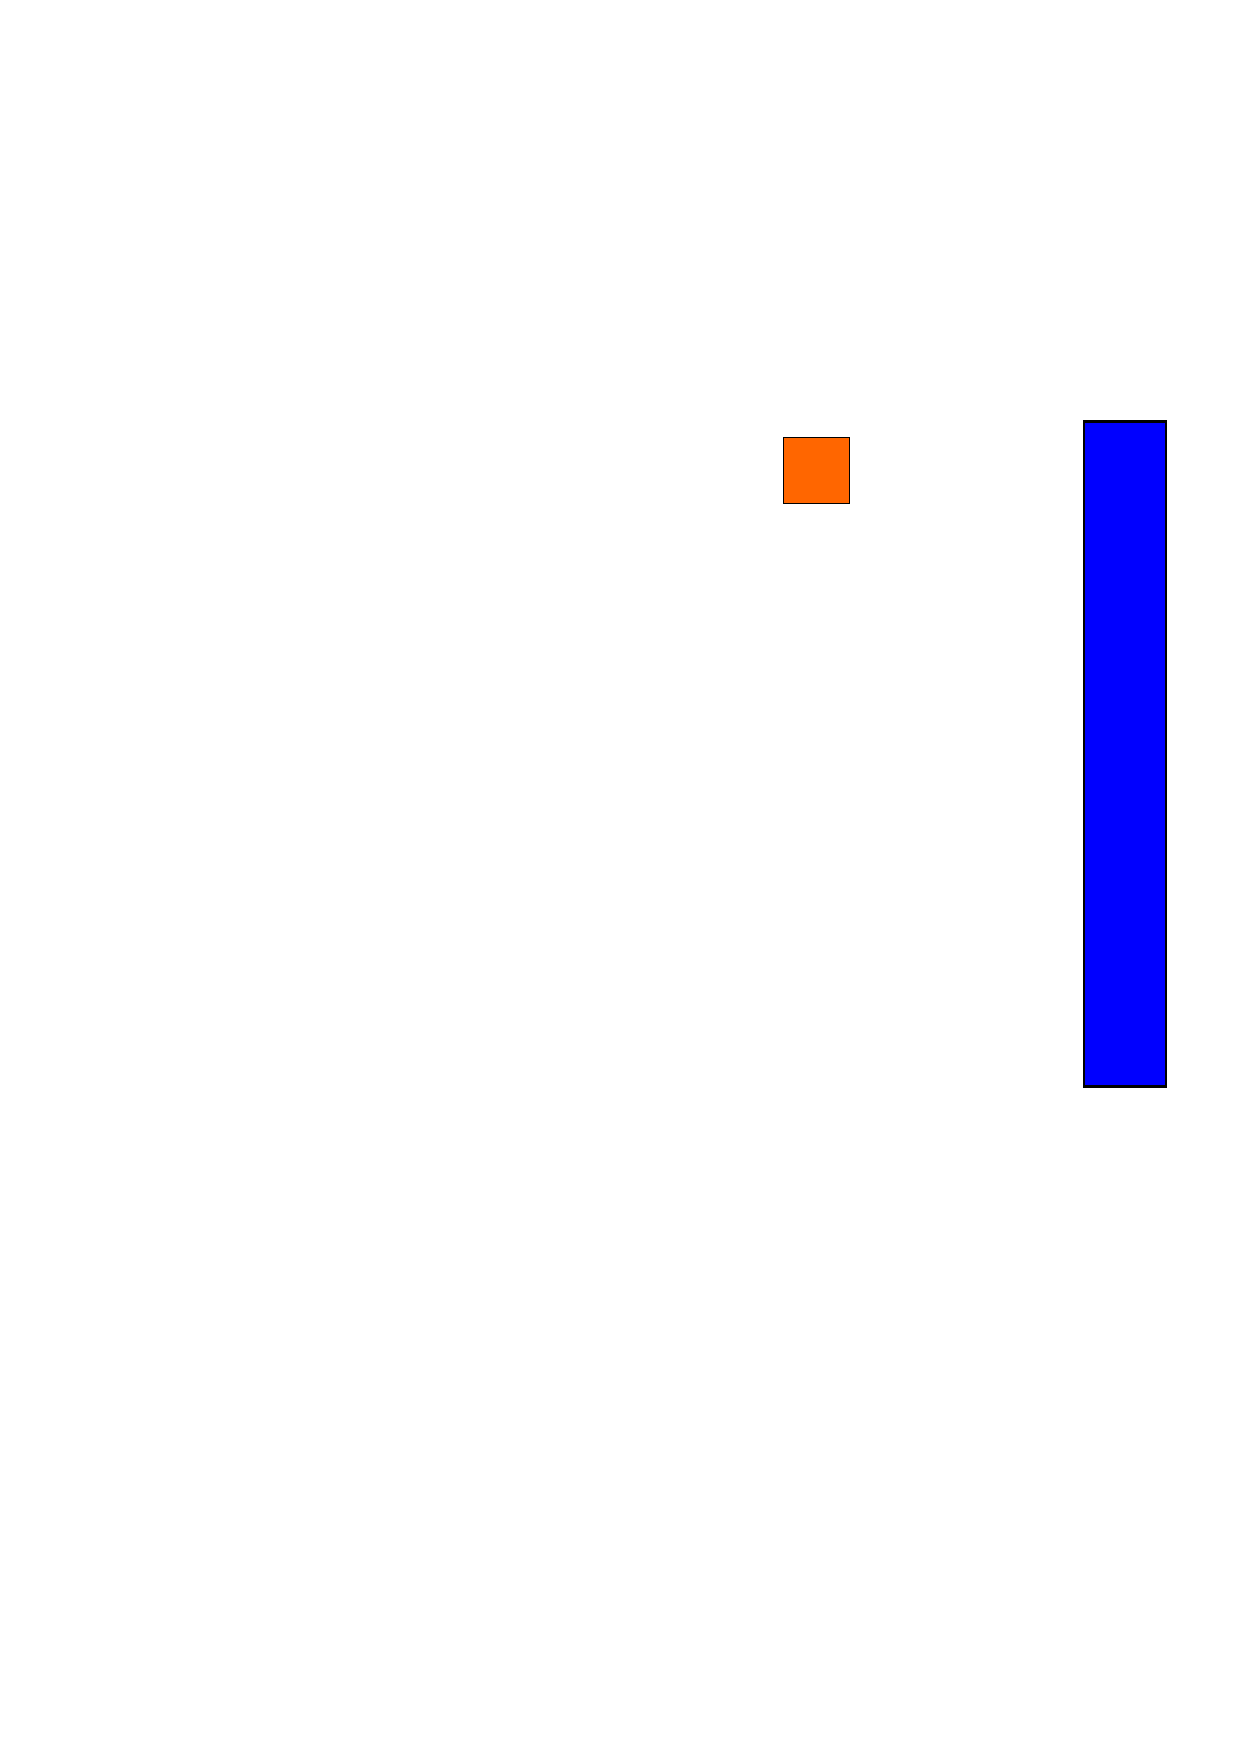
\includegraphics[width=5cm, trim= 0 240 0 100]{img/pong_overlapping_0.pdf}
	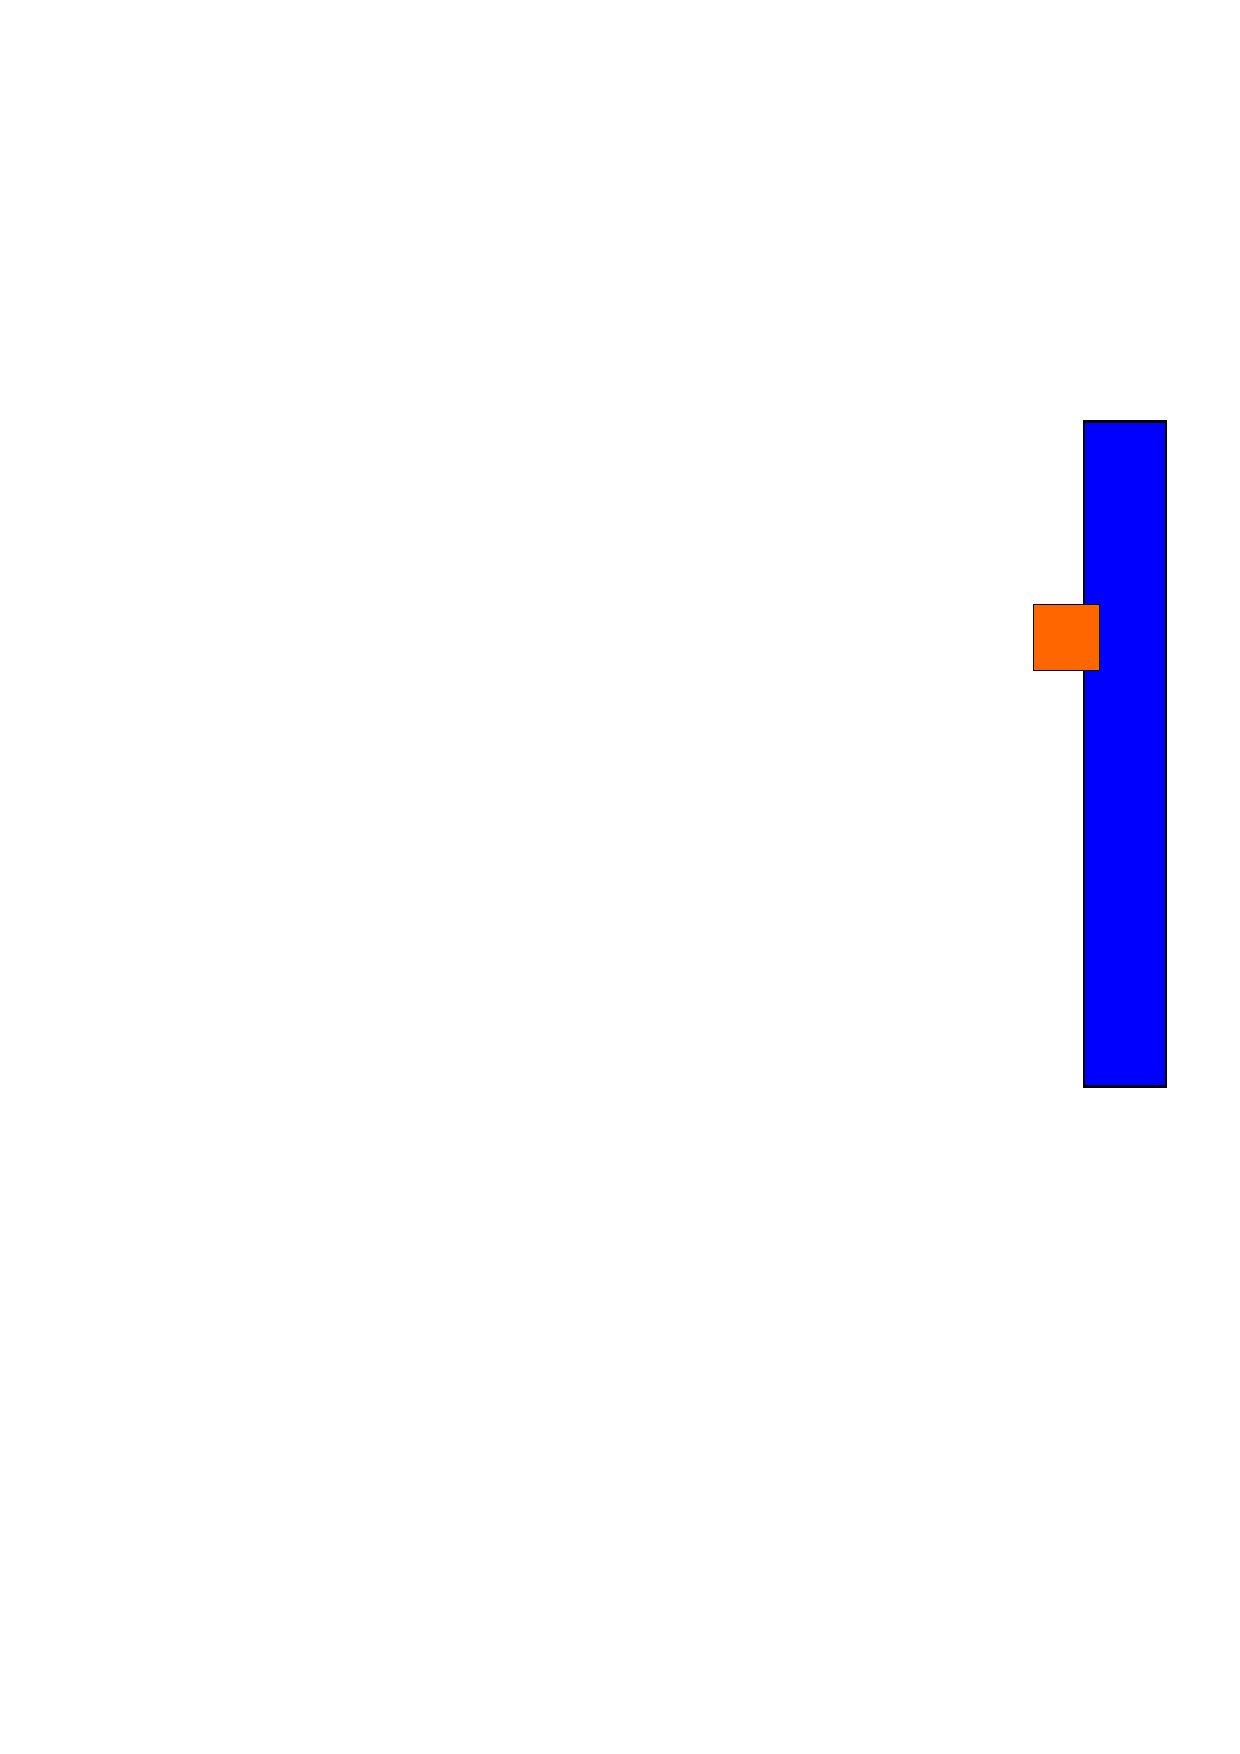
\includegraphics[width=5cm, trim= 0 240 0 100]{img/pong_overlapping_1.pdf}
	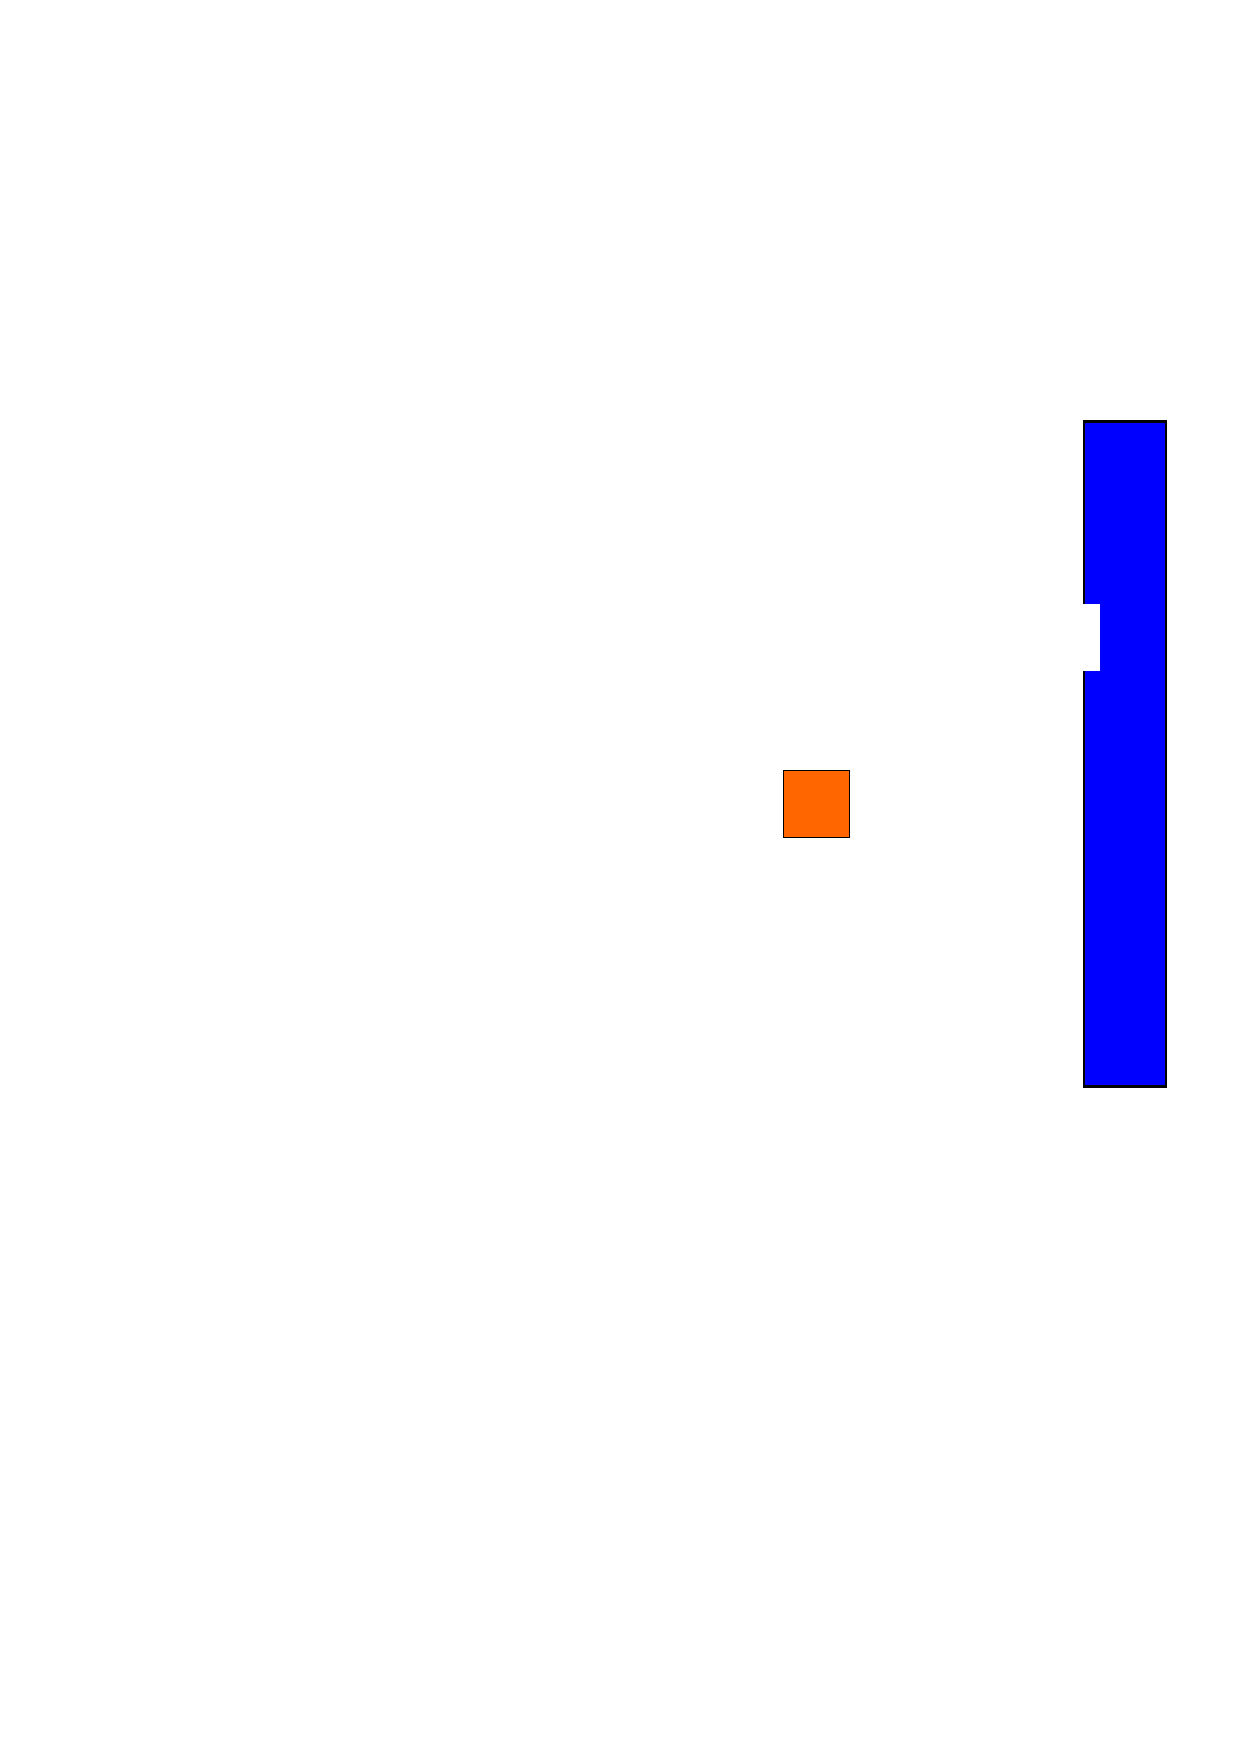
\includegraphics[width=5cm, trim= 0 240 0 100]{img/pong_overlapping_2.pdf}
	
	\caption{Paddle turning blank after overlapping}
\end{figure}
The overlapping occured when the distance between the ball and the player became smaller than the speed in horizontal direction. For example, if the horizontal speed of the ball was 3 pixels, and the distance between the ball and the player was two pixels, the ball would move one pixel into the player leaving a one pixel wide blank area on the player. For a simple game such as Pong, multipe graphic layers are not needed. To prevent overlapping, the ball position would be adjusted so that it stuck to the paddle instead of overlapping. 
\paragraph{math.h}We tried giving the player more control over the ball as it intersected with the paddle. Our plan was to adjust the angle of the ball each time the ball hit the paddle. The closer to the edge of the paddle the ball would hit, the wider the new angle would be. To do this we needed some functions from the standard math library. Including $<math.h>$ would unfortunately not give us acces to theese functions. We did however find a header on the computer that included the required functions, but came across some problems when trying to link it. We tried using the specific address, but then dependencies would not be found for the math header. We tried finding a way to change the \emph{C\_INCLUDE\_PATH} from the makefile for some of the files, while keeping the default setting for the other, but where unsucessfull. As we where supposed to keep our main focus on the driver, a workaround was used. Now we simply change the horizontal speed of the ball when it hits a paddle. 

\subsection{Driver concurrency}
When writing a driver, we need to handle concurrency in the utilization of the driver.
\paragraph{Only on handle allowed}
Using the \vn{device\_open} variable in \mn{driver-gamepad.c}, we made sure that only one handler of the driver could be open at any time. Because the open file operation is protected by a critical region in the Linux kernel, no race conditions can occur setting this variable.\\
\emph{TODO - Finne ut om det er riktig med kritisk region}
\paragraph{Signal mask}
As seen in lines 7-9 of figure \ref{fig:sighandler}, we set a signal mask when assigning signal handlers. By adding signals to this mask, we tell the operating system that these signals should be blocked while the signal handler is running. In this solution, the only code that modifies the game state is signal handlers for \textbf{SIGUSR1} (buttons) and \textbf{SIGALRM} (timer), and by adding these to the signal mask, we guarantee that the signal handlers will run one by one, making it impossible for race conditions and invalid program state.


\subsection{Energy efficiency}
\label{subsection:energy-efficiency}
As we are no longer programming on the "bare metal", we have less control over the software running on the chip. \emph{uClinux} have certain requirements regarding timers and other peripherals, and \cite{compendium} states that "all relevant clocks are already turned on". We therefore concluded that the oscilator setup was fixed (making us unable to experiment with Energy Modes), and had to use other techniques to reduce energy consumption.

\subsubsection{Interrupts and signals}
We implemented our driver so no polling mechanisms were needed (as described in section \ref{subsection:signals-and-interrupts}). As a consequence, the program will stay most of its time in a \emph{pause()} loop, leaving the CPU and IO buses free to do other stuff (or  sleep). This behaviour decreases power consumption.

\subsubsection{Optimizing screen update}
As described in section \ref{subsubsection:framebuffer-update-modes}, we try to limit the area of the screen we update. We have been adviced that tuning this area have an impact on performance and energy efficiency.

\subsubsection{Tickless idle}
\begin{figure}[h]
	\centering
	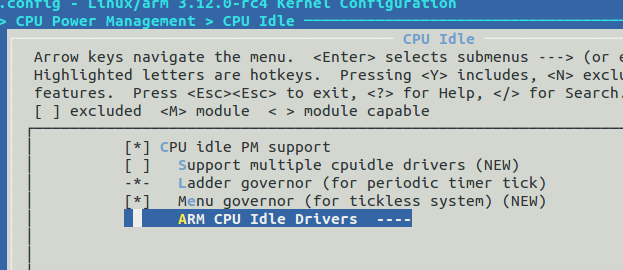
\includegraphics[width=12cm]{img/tickless.png}
	\caption{Configuring the kernel to tickless idle}
	\label{fig:tickless}
\end{figure}
Because our game is handeled entirely by signal handlers, leaving the main program in a pause loop, we wanted to reduce the power consumption while waiting for an interrupt/signal. In order to do that, we were adviced to put the kernel in a mode known as tickless idle. This turns off the normal periodic timer interrupts, which decreases power usage.\\
\\
Tickles idle was enabled in the \emph{kernelconfig} by setting \emph{Idle dynticks system (tickless idle)} in \emph{General setup $\rightarrow$ Timer subsystem $\rightarrow$ Timer tick handling} (see figure \ref{fig:tickless}). This sets the \emph{NO\_HZ\_IDLE} flag.

\subsection{Installation instructions}
